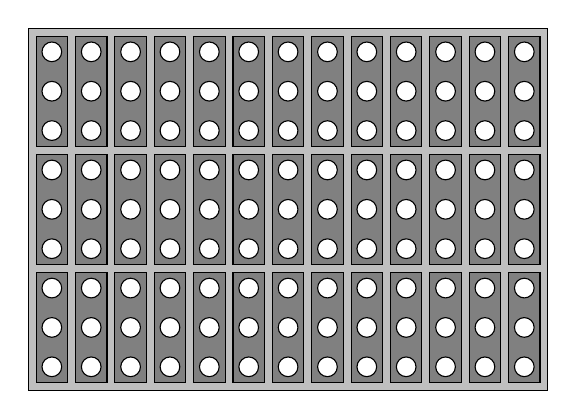
\begin{tikzpicture}[scale=0.5]
\def\dx{1};
\def\dy{1};
\def\r{0.25};
\def\m{0.1};
\filldraw[draw=black,fill=gray!50!white] (-0.5*\dx-\m,-1.5*\dy-\m) rectangle ++(13*\dx+2*\m,9*\dy+2*\m);
\foreach \y in {0,1,2} {
  \foreach \x in {0,...,12} {
    \begin{scope}[xshift=\x*\dx cm,yshift=3*\y*\dy cm]
    \filldraw[draw=black,fill=gray] (-0.5*\dx+\m,-1.5*\dy+\m) rectangle ++(\dx-2*\m,3*\dy-2*\m);
	\foreach \z in {-1,0,1} {
	  \filldraw[draw=black,fill=white] (0,\dy*\z) circle (\r cm);
	}
	\end{scope}
  }
}
\end{tikzpicture}